\chapter{Server}

Dieser Abschnitt beschreibt die Komponenten des Entwurfs des
Kobold Servers. In der Iteratrion 1 untergliedert sich der Server
in 5 Komponenten. Man beachte insbesondere auch das Kapitel 2.3
der Spezifikation1, das die Anforderungen an die jeweiligen
Komponenten spezifiziert.

\section{�berblick}
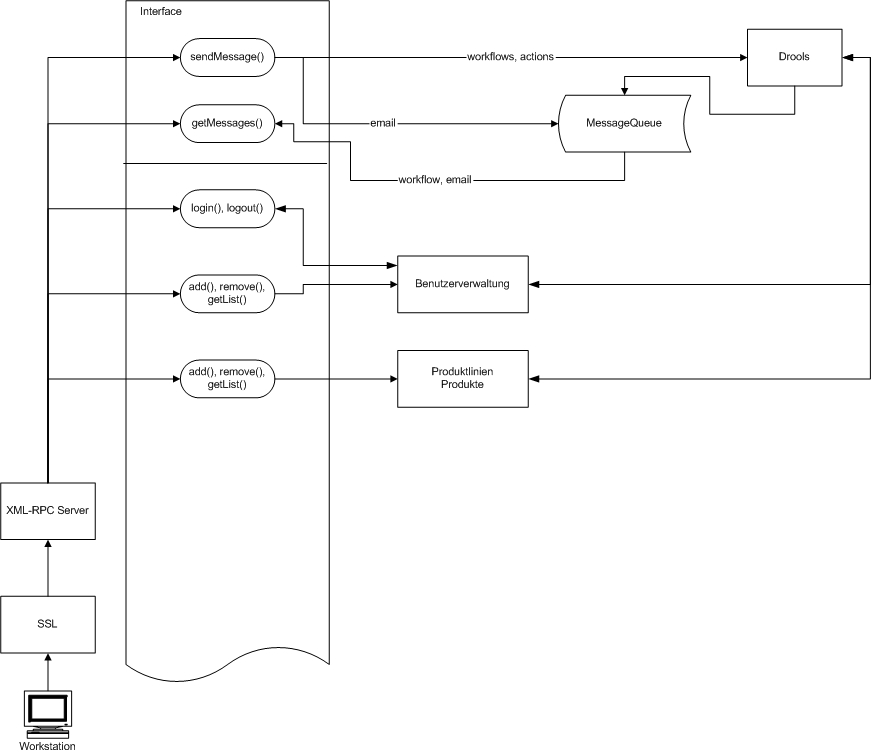
\includegraphics[width=15cm]{server.jpg}

\section{Komponente Kobold Interface}

Die Komponente Interface bildet die Schnittstelle des Kobold
Servers nach aussen und ist dessen Einsprungklasse. Sie wird von
den Kobold Clients �ber remote procedure calls angesprochen.
Anfragen werden an die daf�r zust�ndigen Komponenten des Kobold
Servers delegiert.

\section{Komponente Drools}

Diese Komponente erh�lt Daten �ber durchgef�hrte (VCM-)Actionen
sowie Workflowobjekte, die auf die vorhandenen Regelmengen
angewendet werden. Daf�r k�nnen ben�tigte Daten von den
Komponenten Benutzerverwaltung und Produktlinienverwaltung
abgerufen werden. Als Konsequenz k�nnen Workflows oder EMails an
die MessageQueue-Komponente �bergeben werden.

\section{Komponente MessageQueue}

Aufgabe dieser Komponente ist die Verwaltung und Zustellung von
Worklows und EMails an die addressierten Clients, sobald diese
getMessages() aufrufen.

\section{Komponente Benutzerverwaltung}

Die Benutzerverwaltung ist zust�ndig f�r die Authentifizierung der
Benutzer beim Login und verwaltet deren Rollendaten. S�mtliche
Benutzerdaten k�nnen von dieser Komponente abgefragt werden.

\section{Komponente Produktlinien-/Produktverwaltung}

Diese Komponente verwaltet s�mtliche auf dem Server zu
persistierende Daten zu Produktlinien und Produkten.
